Este capítulo aborda a execução do método proposto por este trabalho e a análise dos resultados obtidos pelos experimentos realizados a fim de verificar a viabilidade do projeto, bem como sua eficiência.

\section{Planejamento dos experimentos}\label{sec:result_planejamento}
O intuito desta avaliação experimental é verificar a capacidade do sistema \theproduct{} classificar as ações do usuário a partir da leitura de sensores, e exibir um objeto 3D animado que demonstra esses dados. Para tal, foi necessário o desenvolvimento de um protótipo físico para a captura dos movimentos e de um \textit{software} para visualização.

\subsection{Captura dos movimentos}\label{sec:result_captura}
O protótipo para captura de dados consiste em um Arduino Nano, um sensor MPU-6050 e um sensor flexível, conectados conforme o esquema da \autoref{fig:result_schem}. 

\begin{figure}[ht]
	\caption{\label{fig:result_schem}Esquema das conexões dos sensores ao Arduino}
	\begin{center}
	    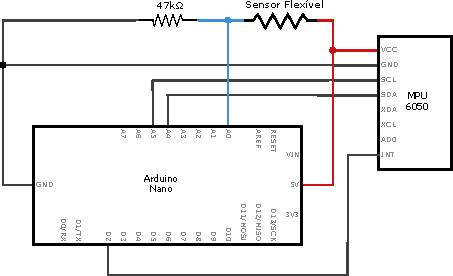
\includegraphics[width=.8\textwidth]{resources/result_schem}
	\end{center}
	\legend{Fonte: Elaborada pelo autor}
\end{figure}

Todos esses equipamentos foram fixados no acessório mostrado na \autoref{fig:result_prototipo}, que pode ser posicionado no joelho do usuário, com o MPU-6050 (b) posicionado acima do joelho, e o sensor flexível (a) posicionado atrás do joelho. Este sensor teve de ser posicionado desta forma devido ao seu comprimento de apenas 2,2 polegadas.

\begin{figure}[ht]
	\caption{\label{fig:result_prototipo}Protótipo com o sensor flexível (a) e o MPU-6050 (b) conectados ao Arduino Nano}
	\begin{center}
	    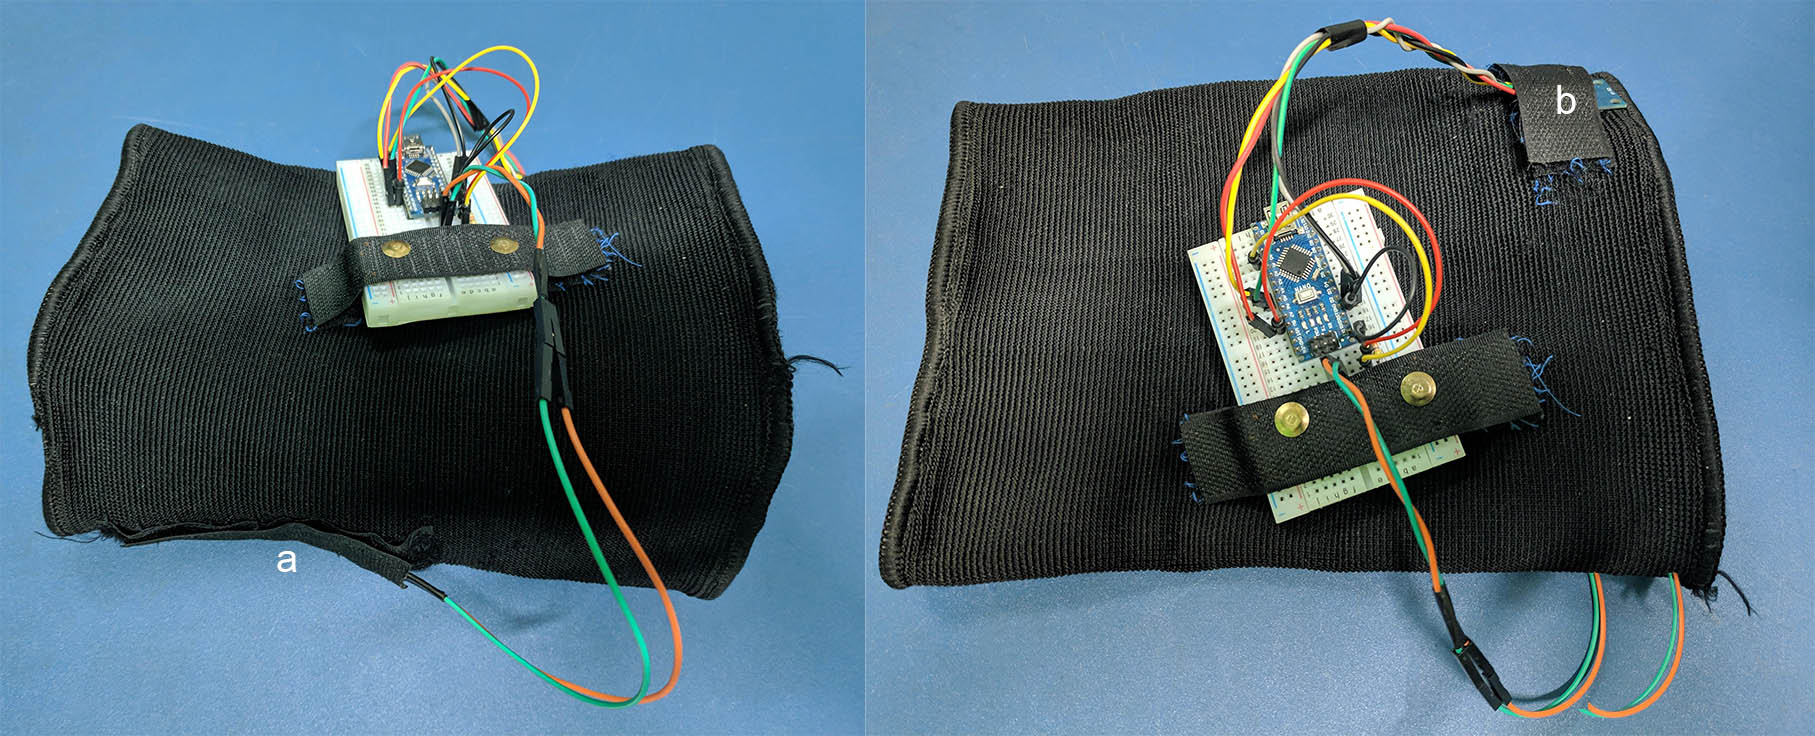
\includegraphics[width=.8\textwidth]{resources/result_prototipo}
	\end{center}
	\legend{Fonte: Elaborada pelo autor}
\end{figure}

Para que sejam possíveis a leitura e a classificação dos dados capturados, o Arduino deve ser conectado via USB em um computador que esteja executando o \textit{software} de simulação. Os dados do giroscópio, acelerômetro e resistência do sensor flexível, respectivamente, são enviados continuamente via comunicação serial pelo \textit{software} carregado no Arduino.

\subsection{\textit{Software} de simulação}\label{sec:result_simulacao}
O sistema de simulação é executado em um computador e foi desenvolvido na linguagem Python, para facilitar o uso da ferramenta scikit-learn. O programa é composto por diversos componentes que se integram para realizar diferentes atividades: leitura dos dados, através da biblioteca \textit{pyserial}\footnote{\url{https://github.com/pyserial/pyserial}}; gravação dos dados em arquivos; classificação dos dados, utilizando scikit-learn; e a exibição 3D com o uso das bibliotecas \textit{PyOpenGL}\footnote{\url{http://pyopengl.sourceforge.net/}} e \textit{pygame}\footnote{\url{https://www.pygame.org/}}.

A simulação animada em 3D, exibida na~\autoref{fig:result_simulacao} mostra em tempo real o movimento realizado pelos dois sensores e, após a captura dos dados, mostra também a ação realizada na prótese simulada, baseado na classificação dos dados de movimento.

\begin{figure}[ht]
	\caption{\label{fig:result_simulacao}Visualização da posição da perna do usuário e simulação da prótese}
	\begin{center}
	   % 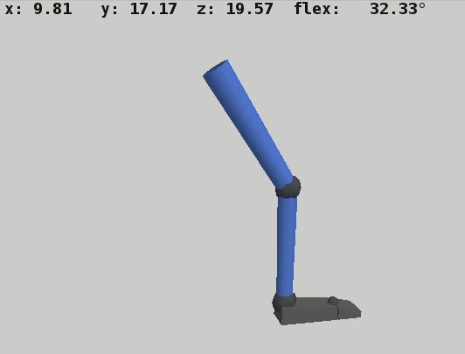
\includegraphics[width=.8\textwidth]{resources/result_simulacao}
	   \missingfigure[figwidth=.8\textwidth]{Screenshot do simulador}
	\end{center}
	\legend{Fonte: Elaborada pelo autor}
\end{figure}

\section{Execução dos experimentos}\label{sec:result_execucao}

\todo[inline]{Dado tal cenário, coletei os dados, funcionou mas poderia melhorar de tal jeito, isso e aquilo. Se não funcionou, pode ter sido limitação do classificador, ou do sensor, ou da placa.}

As ações definidas para este experimento foram apenas voltadas à detecção de uma caminhada plana, classificando cada um dos passos de cada perna\todo{devido à limitação dos sensores disponíveis, pois o giroscópio não é tão preciso assim sozinho (na verdade só não deu tempo mesmo)}{}.

Foram selecionados indivíduos para gerar o conjunto de dados que seria utilizado para a classificação, e solicitado para que cada um deles caminhasse em linha reta, enquanto era capturado o estado da transição de cada uma das ações. A captura foi feita a partir de um cabo USB conectado a um notebook \todo{configuração} estabelecendo conexão via porta serial para o programa.

\subsection{Análise dos resultados}\label{sec:result_analise}

A partir dos dados coletados dos usuários, verificou-se\todo{Falar do KFold} dentre os algoritmos do scikit-learn\todo{Conferir coerência em relação ao nome do scikit em outras partes do texto}{ } que a árvore de decisões CART seria o mais apropriado, com acurácia de aproximadamente 94,7\%.
\todo[inline]{Escolha do algoritmo, comparação de gráficos}
\todo{Corrigir imagem: separar os gráficos ou manter só o de baixo}\begin{figure}[ht]
	\caption{\label{fig:result_accuracy_plot}Gráfico de acurácia}
	\begin{center}
	    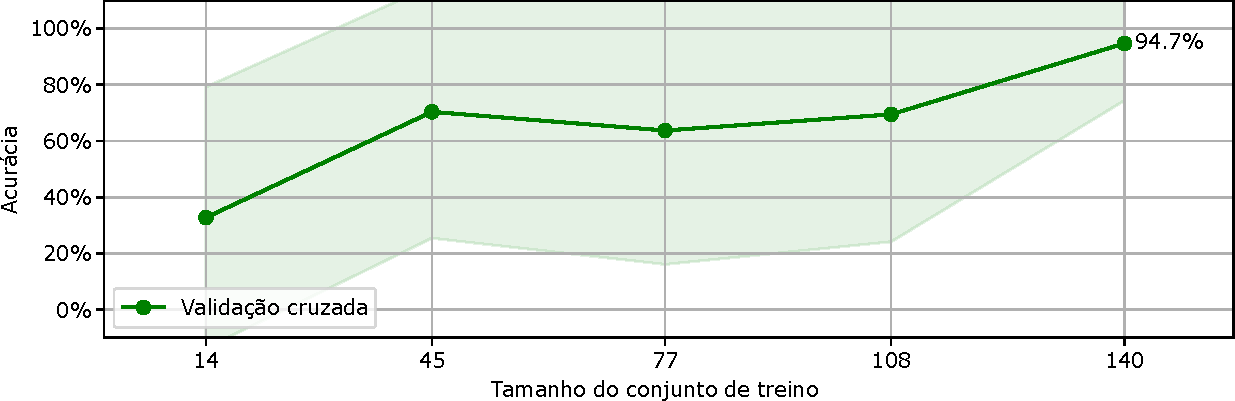
\includegraphics[width=\textwidth]{resources/result_accuracy_plot}
	\end{center}
	\legend{Fonte: Elaborada pelo autor}
\end{figure}

Ao longo dos experimentos realizados, notou-se que o sensor flexível ficou cada vez menos preciso.

Observou-se que com a coleta realizada, não foi possível gerar um conjunto de dados genérico que funcionasse para todos os indivíduos, mas os conjuntos isolados para cada um deles funcionava. \todo{Reformular isso aqui.}